%杨舒云的实验报告编辑界面,使用了Huanyu Shi,2019级的模板,杨舒云在此拜谢ORZ!

%!TEX program = xelatex
\documentclass[dvipsnames, svgnames,a4paper,11pt]{article}
% ----------------------------------------------------- 
%	加边框的命令
%	参考:https://tex.stackexchange.com/questions/531559/how-to-add-the-page-border-for-first-two-pages-in-latex
\usepackage{tikz}
\usetikzlibrary{calc}
\usepackage{eso-pic}
\AddToShipoutPictureBG{%
\begin{tikzpicture}[overlay,remember picture]
\draw[line width=0.6pt] % 边框粗细
    ($ (current page.north west) + (0.6cm,-0.6cm) $)
    rectangle
    ($ (current page.south east) + (-0.6cm,0.6cm) $); % 边框位置
\end{tikzpicture}}


\usepackage{xcolor}
\definecolor{c1}{HTML}{086173} % 目录颜色 原版为2752C9 紫灰色535AAA 蓝紫色0B0DB7 深蓝色070F94 湖绿色219394 松石灰绿086173
\definecolor{c2}{HTML}{E20129} % 引用颜色 原版\definecolor{c2}{RGB}{190,20,83} 橙色F24729

\usepackage{ctex}
\usepackage[top=28mm,bottom=28mm,left=15mm,right=15mm]{geometry}
\usepackage{hyperref} 
\hypersetup{
	colorlinks,
	linktoc = section, % 超链接位置,选项有section, page, all
	linkcolor = c1, % linkcolor 目录颜色
	citecolor = c1  % citecolor 引用颜色
}
\usepackage{amsmath,enumerate,multirow,float}
\usepackage{tabularx}
\usepackage{tabu}
\usepackage{subfig}
\usepackage{fancyhdr}
\usepackage{graphicx}
\usepackage{wrapfig}  
\usepackage{physics}
\usepackage{appendix}
\usepackage{amsfonts}

%
\usepackage{tcolorbox}
\tcbuselibrary{skins,breakable}
\newtcolorbox{tbox}[2][]{
    colframe=black!70!,
    breakable,
    enhanced,
	boxrule =0.5pt,
    title = {#2},
    fonttitle = \large\kaishu\bfseries,
	drop fuzzy shadow,
    #1
}
\newtcolorbox[auto counter,number within=section]{question}[1][]{
  top=2pt,bottom=2pt,arc=1mm,
  boxrule=0.5pt,
%   frame hidden,
  breakable,
  enhanced, %跨页后不会显示下边框
  coltitle=c1!80!gray,
  colframe=c1,
  colback=c1!3!white,
  drop fuzzy shadow,
  title={思考题~\thetcbcounter:\quad},
  fonttitle=\bfseries,
  attach title to upper,
  #1
}

% ---------------------------------------------------------------------
%	利用cleveref改变引用格式,\cref是引用命令
\usepackage{cleveref}
\crefformat{figure}{#2{\textcolor{c2}{Figure #1}}#3} % 图片的引用格式
\crefformat{equation}{#2{(\textcolor{c2}{#1})}#3} % 公式的引用格式
\crefformat{table}{#2{\textcolor{c2}{Table #1}}#3} % 表格的引用格式


% ---------------------------------------------------------------------
%	页眉页脚设置
\fancypagestyle{plain}{\pagestyle{fancy}}
\pagestyle{fancy}
\lhead{\kaishu 中山大学物理与天文学院\uppercase\expandafter{\romannumeral1}} % 左边页眉,学院 + 课程
\rhead{\kaishu 杨舒云的实验报告} % 右边页眉,实验报告标题
\cfoot{\thepage} % 页脚,中间添加页码


% ---------------------------------------------------------------------
%	对目录、章节标题的设置
\renewcommand{\contentsname}{\centerline{\huge 目录}}
\usepackage{titlesec}
\usepackage{titletoc}
% \titleformat{章节}[形状]{格式}{标题序号}{序号与标题间距}{标题前命令}[标题后命令]
\titleformat{\section}{\centering\LARGE\songti}{}{1em}{}

% ---------------------------------------------------------------------
%   listing代码环境设置
\usepackage{listings}
\lstloadlanguages{python}
\lstdefinestyle{pythonstyle}{
backgroundcolor=\color{gray!5},
language=python,
frameround=tftt,
frame=shadowbox, 
keepspaces=true,
breaklines,
columns=spaceflexible,                   
basicstyle=\ttfamily\small, % 基本文本设置,字体为teletype,大小为scriptsize
keywordstyle=[1]\color{c1}\bfseries, 
keywordstyle=[2]\color{Red!70!black},   
stringstyle=\color{Purple},       
showstringspaces=false,
commentstyle=\ttfamily\scriptsize\color{green!40!black},%注释文本设置,字体为sf,大小为smaller
tabsize=2,
morekeywords={as},
morekeywords=[2]{np, plt, sp},
numbers=left, % 代码行数
numberstyle=\it\tiny\color{gray}, % 代码行数的数字字体设置
stepnumber=1,
rulesepcolor=\color{gray!30!white}
}




% ---------------------------------------------------------------------
%	其他设置
\def\degree{${}^{\circ}$} % 角度
\graphicspath{{./images/}} % 插入图片的相对路径
\allowdisplaybreaks[4]  %允许公式跨页 
\usepackage{lipsum}
\usepackage{adjustbox}
%\usepackage{mathrsfs} % 字体
\captionsetup[figure]{name=Figure} % 图片形式
\captionsetup[table]{name=Table} % 表格形式

\begin{document}
	
	
	
	% 实验报告封面	
	
	% 顶栏
	\begin{table}
		\renewcommand\arraystretch{1.7}
		\begin{tabularx}{\textwidth}{
				|X|X|X|X
				|X|X|X|X|}
			\hline
			\multicolumn{2}{|c|}{预习报告}&\multicolumn{2}{|c|}{实验记录}&\multicolumn{2}{|c|}{分析讨论}&\multicolumn{2}{|c|}{总成绩}\\
			\hline
			\LARGE25 & & \LARGE30 & & \LARGE25 & & \LARGE80 & \\
			\hline
		\end{tabularx}
	\end{table}
	% ---
	
	% 信息栏
	\begin{table}
		\renewcommand\arraystretch{1.7}
		\begin{tabularx}{\textwidth}{|X|X|X|X|}
			\hline
			年级、专业: & 2022级 物理学 &组号: & 2\\
			\hline
			姓名: & 杨舒云  & 学号: & 22344020\\
			\hline
			实验时间: & 2024/3/14 & 教师签名: & \\
			\hline
		\end{tabularx}
	\end{table}
	% ---
	
	% 大标题
	\begin{center}
		\LARGE Lab2-2 \quad 迈克尔干涉实验(白光干涉)
	\end{center}
	% ---
	
	% 注意事项
	
	% 基本
	\textbf{【实验报告注意事项】}
	\begin{enumerate}
		\item 实验报告由三部分组成:
		\begin{enumerate}
			\item 预习报告:课前认真研读实验讲义,弄清实验原理;实验所需的仪器设备、用具及其使用、完成课前预习思考题;了解实验需要测量的物理量,并根据要求提前准备实验记录表格(可以参考实验报告模板,可以打印)。\textcolor{red}{\textbf{(20分)}}
			\item 实验记录:认真、客观记录实验条件、实验过程中的现象以及数据。实验记录请用珠笔或者钢笔书写并签名(\textcolor{red}{\textbf{用铅笔记录的被认为无效}})。\textcolor{red}{\textbf{保持原始记录,包括写错删除部分,如因误记需要修改记录,必须按规范修改。}}(不得输入电脑打印,但可扫描手记后打印扫描件);离开前请实验教师检查记录并签名。\textcolor{red}{\textbf{(30分)}}
			\item 数据处理及分析讨论:处理实验原始数据(学习仪器使用类型的实验除外),对数据的可靠性和合理性进行分析;按规范呈现数据和结果(图、表),包括数据、图表按顺序编号及其引用;分析物理现象(含回答实验思考题,写出问题思考过程,必要时按规范引用数据);最后得出结论。\textcolor{red}{\textbf{(30分)}}
		\end{enumerate}
		\textbf{实验报告就是将预习报告、实验记录、和数据处理与分析合起来,加上本页封面。\textcolor{red}{(80分)}}
		\item 每次完成实验后的一周内交\textbf{实验报告}(特殊情况不能超过两周)。
	\end{enumerate}
	
	% 安全
	\textbf{【实验安全注意事项】}	
	\begin{enumerate}
		\item 实验过程中,光源不要随意打开关闭;
		\item 严禁用手触光学镜头的表面;
		\item 严禁用强力和斜向力旋转测微头,这样会损坏测微头或其他部件;
		\item 不要拆卸传动机构,以免影响仪器正常使用;
		\item 实验过程中,数条纹时,避免桌面的振动。
	\end{enumerate}
	
	% ---
	
	% 特别鸣谢
	\textbf{【特别鸣谢及模板说明】}	
	
	感谢2019级学长石寰宇为本实验报告提供\LaTeX 模板。%\textcolor{red}{\textbf{由于原实验报告模板缺少实验编号,为方便在电脑上整理,故添加自命名编号LabX5}}
	% ---
	
	
	
	% 目录
	\clearpage
	\tableofcontents
	\clearpage
	% ---
	
	
	
	% 预习报告	
	
	% 小标题
	\setcounter{section}{0}
	\section{Lab2-2 迈克尔干涉实验(白光干涉) \quad\heiti 预习报告}
	% ---
	
	% 实验目的
	\subsection{实验目的}
	\begin{enumerate}
		\item 观察等倾、等厚干涉现象及调节白光干涉条纹;
		\item 学习用迈克尔逊干涉仪测量钠光谱波长差的方法;
		\item 学习用白光干涉测量透明薄片折射率的方法;
		\item 用迈克尔逊干涉仪测量多种光源的相干长度;
	\end{enumerate}
	% ---
	
	% 仪器用具
	\subsection{仪器用具}
	\begin{table}[htbp]
		\centering
		\renewcommand\arraystretch{1.6}
		% \setlength{\tabcolsep}{10mm}
		\begin{tabular}{p{0.05\textwidth}|p{0.20\textwidth}|p{0.05\textwidth}|p{0.5\textwidth}}
			\hline
			编号& 仪器用具名称 & 数量 &  主要参数(型号,测量范围,测量精度等) \\
			\hline
			1& 精密干涉仪 & 1 & SGM-3 \\
			\hline
			2& He-Ne 激光器 & 1 & -- \\
			\hline
			3& 钠钨双灯 & 1 & -- \\
			\hline
			4& 汞灯 & 1 & -- \\
			\hline
			5& 透明薄片 & 1 & -- \\
			\hline
			6& 螺旋测微计 & 1 & -- \\
			\hline
		\end{tabular}
	\end{table}
	% ---
	
	% 原理概述
	\subsection{原理概述}
	
	\begin{figure}[htbp]
		\centering
		\subfloat[]{
			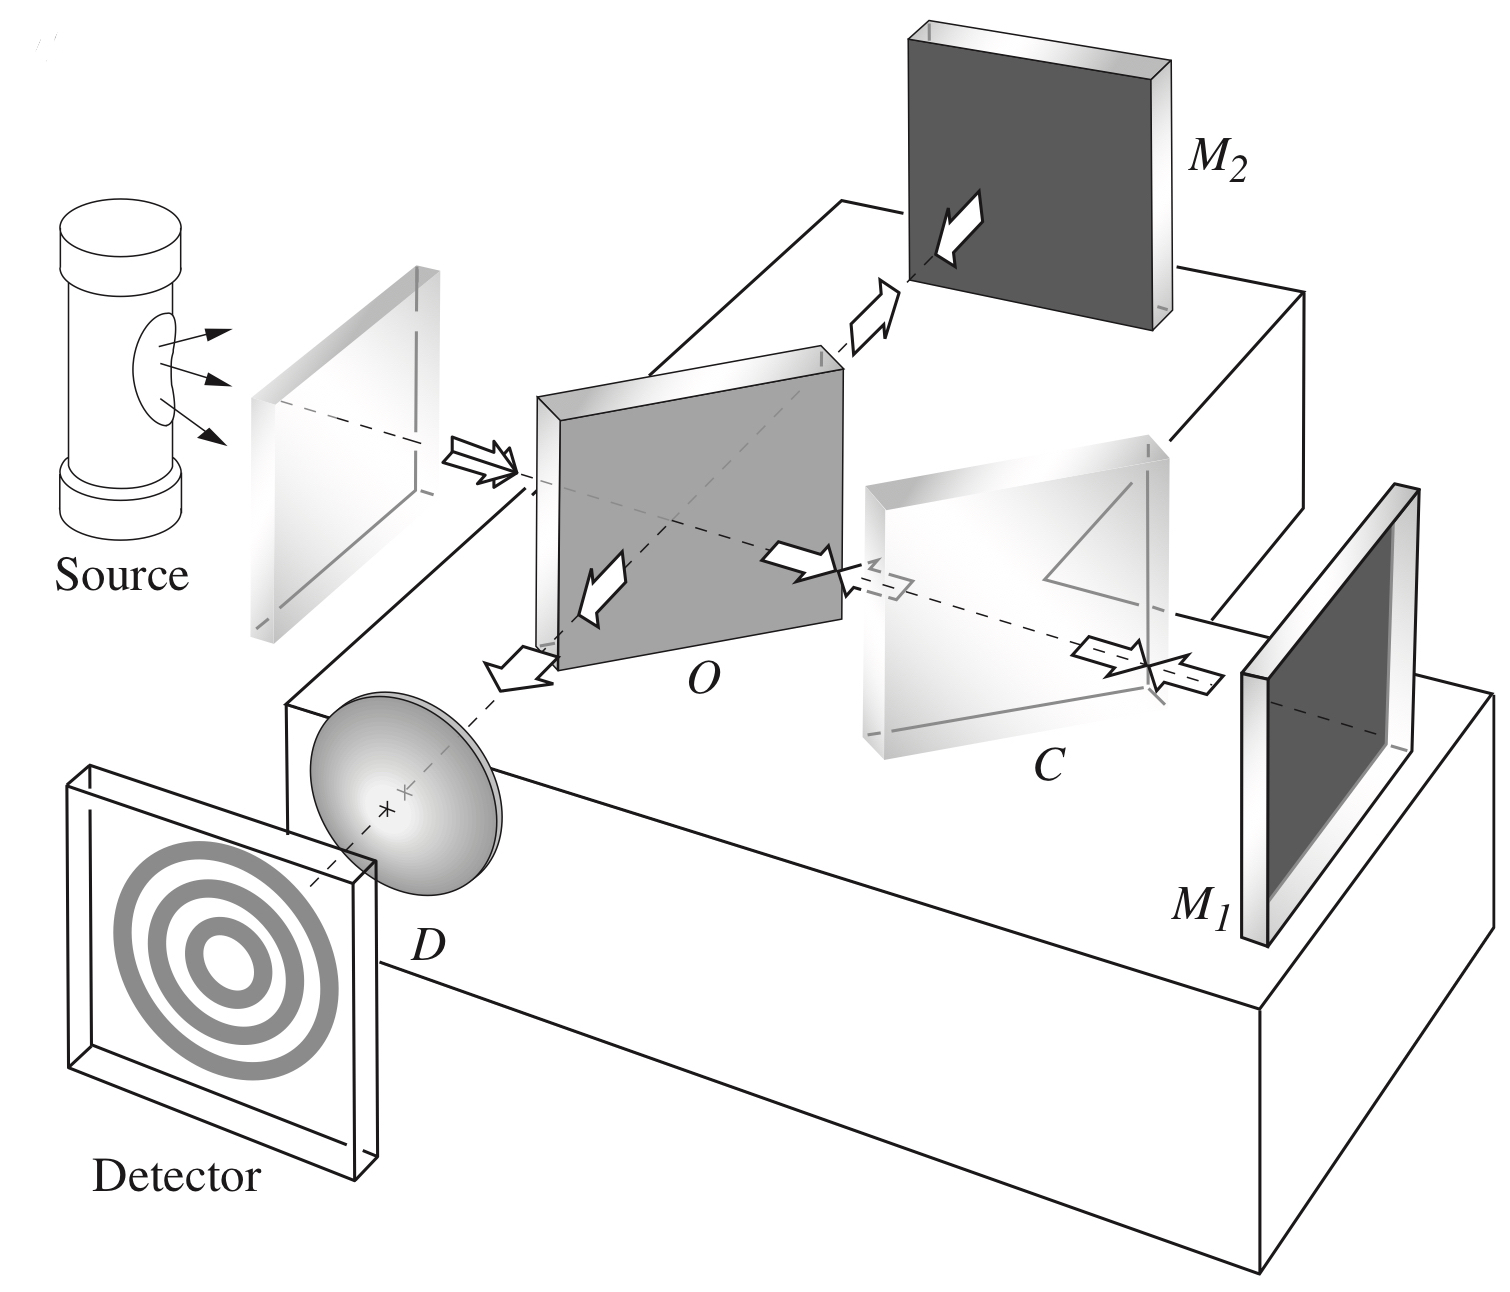
\includegraphics[width=0.3\textwidth]{CB1Graph1.png}
		}
		\subfloat[]{
			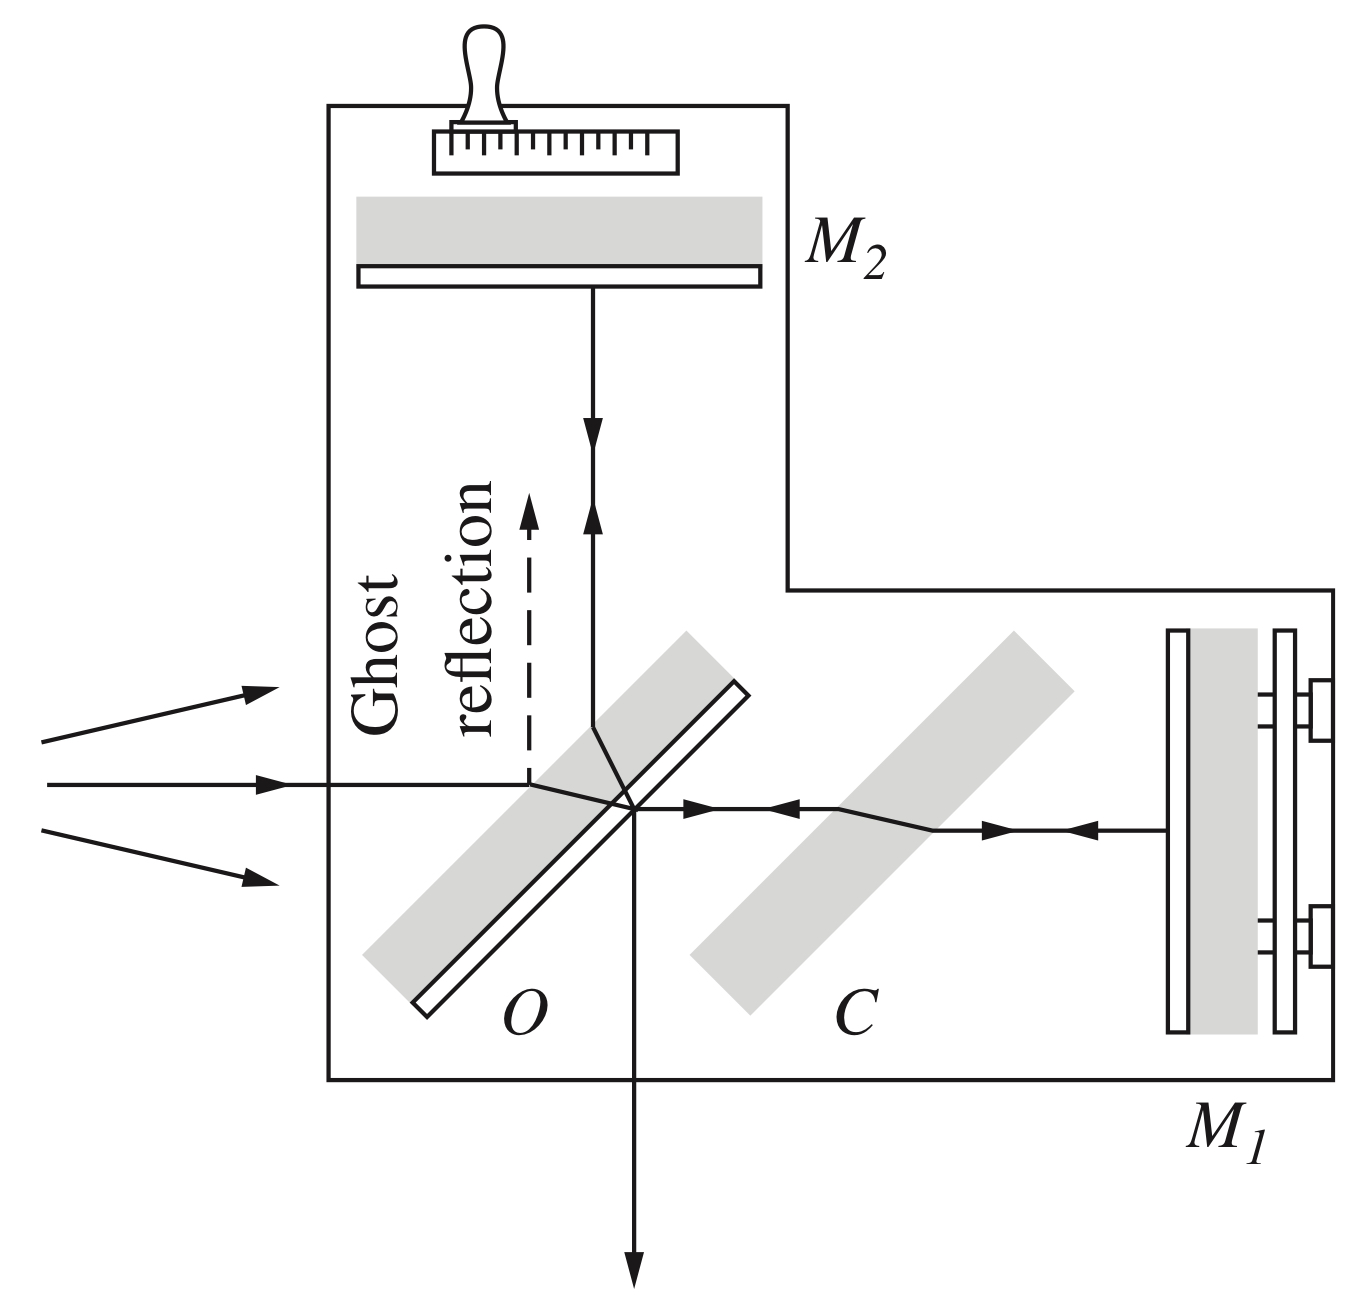
\includegraphics[width=0.3\textwidth]{CB1Graph2.png}
		}
		\caption{迈克尔逊干涉仪光路图}
		\label{fig:figCB1}			
	\end{figure}
	
	\subsubsection{测钠双黄线的波长差}
	\begin{enumerate}
		\item 钠双黄线由两种波长相近的光组成,分别为589.0 nm和589.6 nm。这两条谱线在使用钠灯作为光源时形成各自的干涉条纹,当这些条纹在视场中叠加时,由于波长的差异,会产生错位现象。
		\item 光拍现象是指当两组波长不同的干涉条纹叠加时,随着光程差的变化,干涉条纹出现由清晰到模糊再到清晰的周期性变化过程。这种现象反映了不同波长光线干涉加强或减弱的周期性变化。
		\item 当两束光(具有不同波长)在观察屏上相遇并叠加时,由于它们的波长不同,会导致干涉条纹出现周期性的清晰和模糊变化。当移动反射镜(改变光程差)时,某一波长的亮条纹可能与另一波长的暗条纹重合,导致干涉条纹模糊,反之亦然。通过记录干涉条纹从模糊到清晰再到模糊的变化过程中,反射镜移动的距离,可以计算出两种波长的差值。
		\item \textbf{测量原理}
		
		\begin{figure}[htbp]
			\centering
			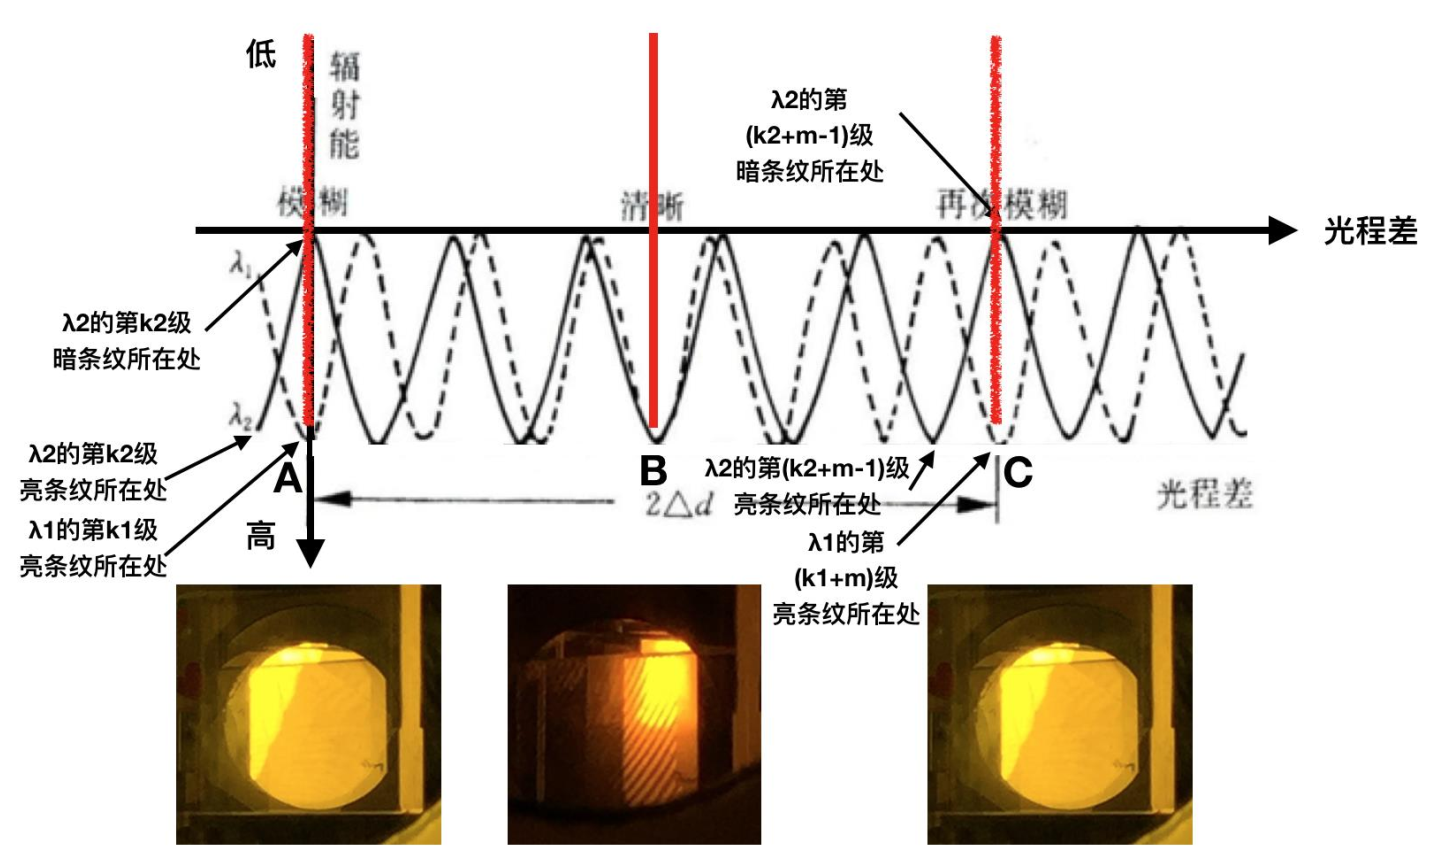
\includegraphics[width=0.8\textwidth]{Lab2_2Gra1.png}
			\caption{“光拍”现象及其原理}
			\label{fig:fig1}
		\end{figure}
		
		在移动反射镜M1时,形成的干涉条纹会从模糊到请晰再到模糊。对波长为$\lambda_{1}$的入射光,当$L_{1}=k_{1}\lambda_{1}$时,在视场巨中处涉加强;在视场E中小处干涉减弱。继续调节M1,当成像出现第一次模糊时,有
		$L _{A}=k_{1}\lambda_{1}=(k_{2}+\frac{1}{2})\lambda_{2}$
		再继续调节,待成像清晰有$L_{C}=(k_{1}+m)\lambda_{1}=[k_{2}+m-1+\frac{1}{2}]\lambda_{2}$
		作差得出$\lambda_{2}-\lambda_{1}=\frac{\lambda_{2}}{m}$
		最终得:
		\[\Delta\lambda=\lambda_{2}-\lambda_{1}=\frac{\lambda_{2}\lambda_{1}}{2\Delta d}=\frac{\bar{\lambda}^{2}}{2\Delta d}\]
		其中,$\bar{\lambda}=\dfrac{\lambda_1+\lambda_2}{2}$为双黄线平均波长。
		
		\textbf{记录下干涉条纹出现一次“模糊-清晰-模糊”的变化时,反射镜 M1 移动的距离$\Delta d$,结合钠双黄线的平均波长,即可利用上式求得钠双黄线的波长差。}
	\end{enumerate}
	\subsubsection{白光干涉的调节,并测定透明薄片的厚度 t 或者折射率 n}
	\begin{enumerate}
		\item 测量原理总结
		\begin{enumerate}
			\item 换上扩散的白光光源(本实验中采用溴钨灯加毛玻璃代替), 微调 M1 精密测微头, 此时应能在玻璃镜(视场) 中观察到彩色的条纹,此即为“白光等厚干涉条纹”。 在视场中心处的彩色条纹之间还可观察到一条全黑的条纹,称为“中心暗纹”。
			\item 然后在反射镜 M1 与分束镜 P1之间放上折射率为 n,厚度为 t 的透明薄片,且尽量使薄片与 M1 镜平行,则此时两干涉臂的光程差要比原来增大。
			\item 放上透明薄片后,透过观察屏玻璃观察透明薄片处,可以看到视场中的白光干涉彩色条纹消失。此时如果将反射镜 M1 镜向前朝分束镜 P1方向移动一段距离$\Delta d$, 使得$\Delta d$ = $\Delta L$ /2(此时候相当于虚光源 S1’和 S2’距离减小 2$\Delta d$ = $\Delta L$,刚好是插入透明薄片后增加的光程差), 则白光彩色干涉条纹重新出现(注意要调节反射镜M1 镜的精密测微头,使得中心暗纹移到视场中央)。此时有
			\[\Delta d=t(n-1)\]
			\item \textbf{测出 M1 镜的移动量$\Delta d$, 若已知透明薄片的厚度 t, 则可由上式可求出透明薄片的折射率n;反之,若已知透明薄片的折射率 n,可求出透明薄片的厚度 t 。}
		\end{enumerate}
		
		\item 重点内容总结
		\begin{enumerate}
			\item \textbf{白光干涉的产生}
			
			撤掉He-Ne激光器并安装白光光源,通过精密调整可移动反射镜$M1$的位置,可以观察到彩色的干涉条纹。这些条纹是由于白光中包含的各种颜色的光波长不同,干涉条件各不相同所致。在干涉图样中,只有波长非常接近的光才能形成明显的干涉条纹,因此白光干涉条纹中心附近会出现一条明显的暗纹,称为“中心暗纹”。
			
			\item \textbf{透明薄片的插入与测量}
			
			在反射镜$M1$与分束镜$P1$之间插入一块已知折射率$n$或已知厚度$t$的透明薄片。由于薄片的插入改变了一个干涉臂的光程,这导致干涉条纹发生移动。通过调节反射镜$M1$,可以将干涉条纹调整至最初的位置,此时通过测量$M1$镜的移动距离$\Delta d$,可以计算出薄片的厚度$t$或折射率$n$。
			
			\item \textbf{计算公式}
			
			根据干涉原理,两干涉臂的光程差变化$\Delta L$可以表示为透明薄片引起的光程改变,即
			\[ \Delta L = 2t(n-1) \]
			其中,$t$是薄片的厚度,$n$是薄片的折射率。若已知薄片的厚度$t$,则可通过测量光程差的变化$\Delta L$来计算薄片的折射率$n$。反之,若已知薄片的折射率$n$,则可通过$\Delta L$计算薄片的厚度$t$。实际操作中,$\Delta L$可以通过测量反射镜$M1$移动的距离$\Delta d$来确定,因为反射镜移动$\Delta d$导致光程差变化为$2\Delta d$(来回路径)。因此,可以得到
			\[ n = 1 + \frac{\Delta L}{2t} = 1 + \frac{\Delta d}{t} \]
			或
			\[ t = \frac{\Delta d}{n-1} \]
		\end{enumerate}
	\end{enumerate}
	% ---
	
	
	
	% 实验前思考题
	\subsection{实验前思考题}
	
	% 思考题1
	\begin{question}
		如何测量透明溶液的折射率?请自行就相关实验原理进行调研,并设计合理试验方案。
	\end{question}
	\begin{enumerate}
		\item 调研记录
		\begin{enumerate}
			\item \textbf{CCD法测量透明介质的折射率}:依据折射定律,设计了一种测量装置,可用于测量透明介质的折射率。该研究详细阐述了测量装置的设计原理、使用方法以及一些实验内容,并给出了一些材料的折射率测量结果 [(Zhang Chang-yi, 2006)]。
			
			\item \textbf{利用CCD测量透明材料折射率的实验方法}:描述了一种基于扩展和准直激光束干涉的透明材料折射率测量实验方法。该光学排列简单易操作,测量折射率的准确性达到了$10^{-3}$的级别,通过应用CCD,这种方法可以扩展到测量其他与折射率相关的系数 [(Deng Guang, 2003)]。
			
			\item \textbf{基于数字全息显微术的溶液折射率测量}:提出了一种基于数字全息显微术的溶液折射率(RI)测量新方法。实验系统由改良的Mach-Zehnder干涉仪和相关的实验室开发分析软件组成。该方法能够高精度地获得被测试溶液的高质量数字全息图,进而计算出溶液的折射率,比用阿贝折射仪测量的结果更准确 [(Sujuan Huang et al., 2017)]。
			
			\item \textbf{非侵入式技术测量清澈和透明液体的折射率}:提出了一种测量清澈和透明液体折射率的光学技术。该技术通过测量光束经过液体介质后发生的横向位移来感知液体折射率的变化。实验结果表明,该技术能够以$10^{-4}$的精度测量折射率,且具有简单和非侵入式的新颖性 [(H. Singh et al., 2014)]。
			
		\end{enumerate}
		
		\begin{figure}[htbp]
			\centering
			\subfloat[]{
				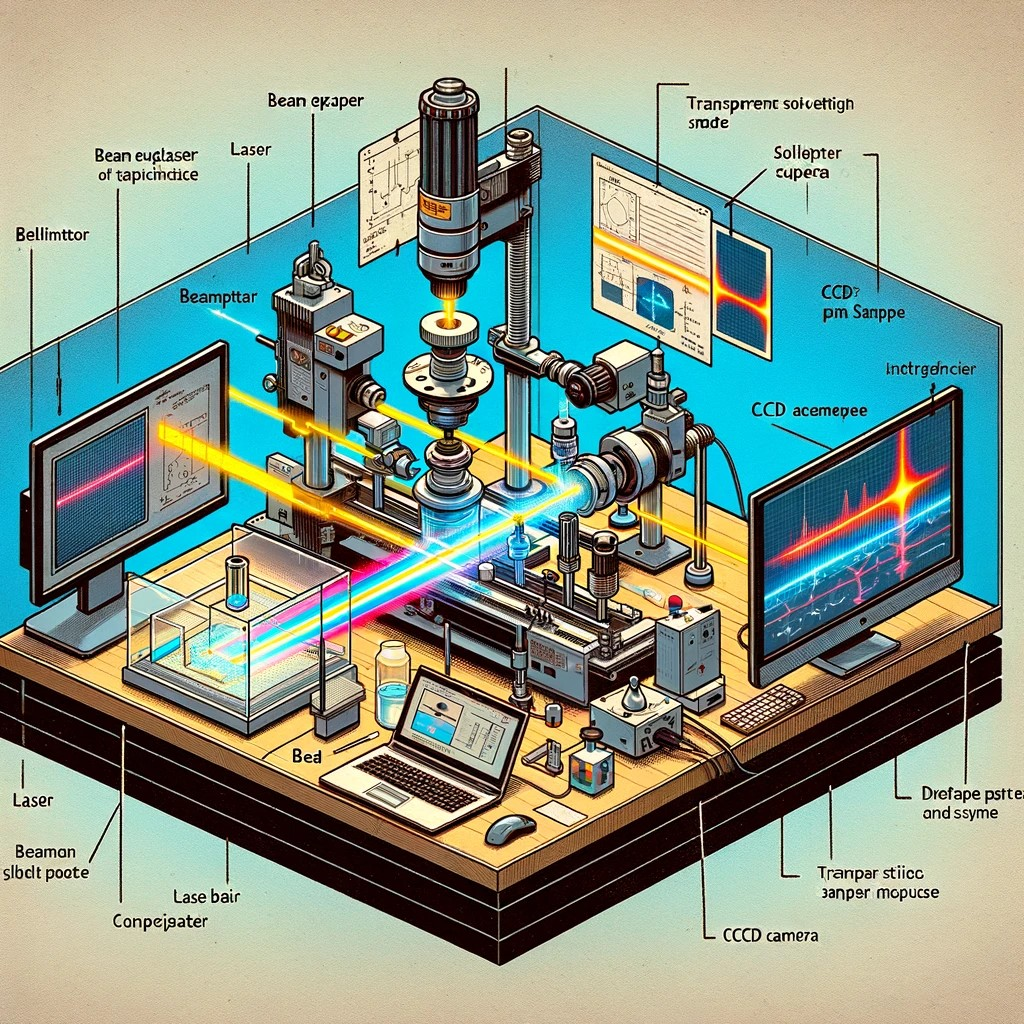
\includegraphics[width=0.4\textwidth]{Lab2_2Gra2.jpg}
			}
			\subfloat[]{
				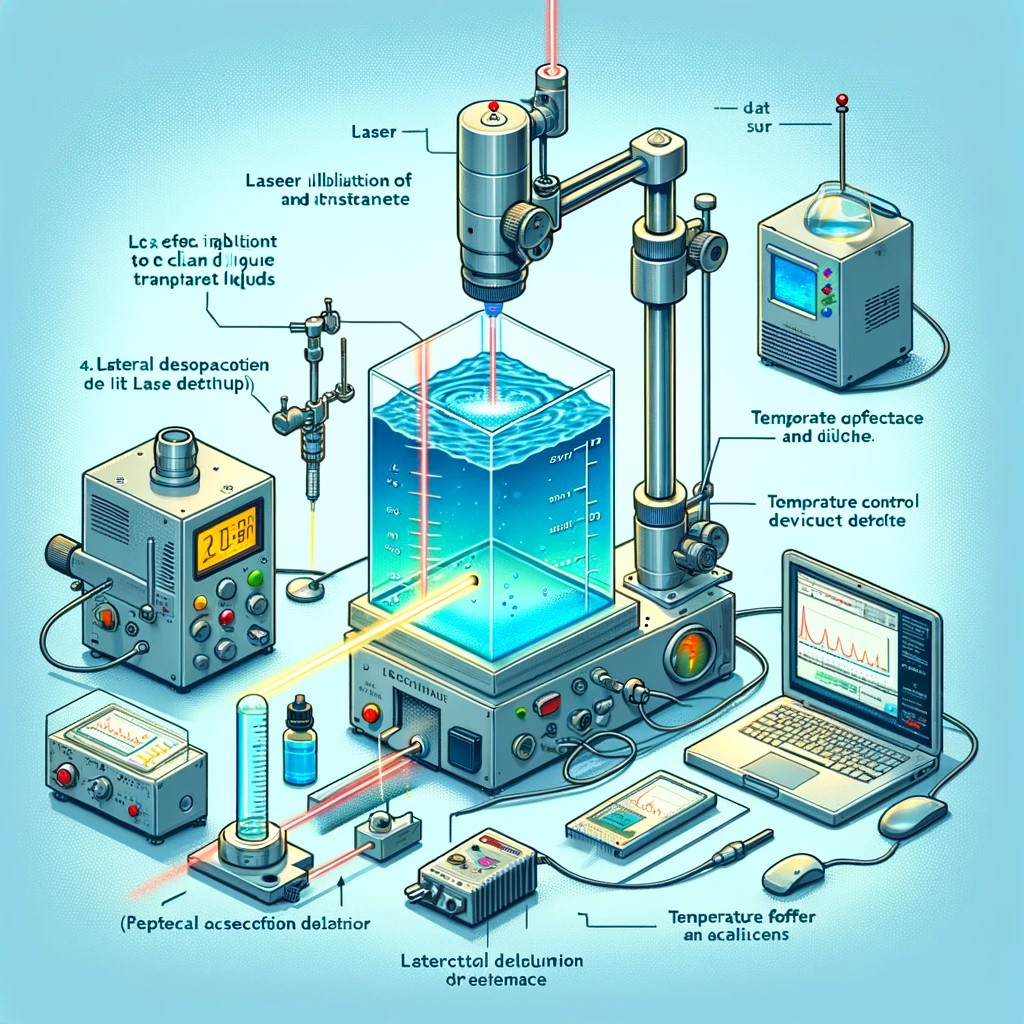
\includegraphics[width=0.4\textwidth]{Lab2_2Gra3.jpg}
			}
			\caption{迈克尔逊干涉仪光路图}
			\label{fig:fig2}			
		\end{figure}
		
		\item 方案设计1
		
		基于CCD法测量透明介质的折射率。
		
		\begin{enumerate}
			\item \textbf{实验材料与设备:}
			
			\begin{itemize}
				\item 激光器(例如:He-Ne激光器)
				\item CCD相机
				\item 计算机(带有图像处理和数据分析软件)
				\item 透明溶液样品
				\item 标准折射率已知的透明溶液(用于校准)
				\item 光学平台(包括固定装置和光路调整设备)
				\item 分光镜
				\item 光束扩展器
				\item 准直镜
			\end{itemize}
			
			\item \textbf{实验步骤:}
			
			\begin{enumerate}
				\item 设备安装与校准:
				\begin{itemize}
					\item 将激光器安装在光学平台上,并使用光束扩展器和准直镜确保发出的激光束是准直的。
					\item 安装分光镜,将激光束分成两路,一路直接照射CCD相机,另一路经过待测溶液后再照射CCD相机。
					\item 使用已知折射率的标准溶液进行系统校准,确保测量系统的准确性。
				\end{itemize}
				
				\item 溶液准备:
				\begin{itemize}
					\item 将待测透明溶液装入透明的容器中,确保容器壁厚均匀,无色差和畸变。
					\item 调整容器位置,使激光束能够穿过溶液并最终到达CCD相机。
				\end{itemize}
				
				\item 数据采集:
				\begin{itemize}
					\item 开启激光器和CCD相机,记录穿过标准溶液和待测溶液的激光束生成的干涉图案。
					\item 使用图像处理软件分析干涉图案,收集干涉条纹的变化数据。
				\end{itemize}
				
				\item 数据分析:
				\begin{itemize}
					\item 根据干涉图案的变化,利用软件计算待测溶液的折射率。可以通过比较标准溶液和待测溶液的干涉图案变化,计算出待测溶液的折射率。
				\end{itemize}
				
				\item 结果验证:
				\begin{itemize}
					\item 使用不同浓度的已知折射率溶液验证测量系统的准确性和重复性。
					\item 必要时,调整实验设置或重新校准系统,以提高测量结果的准确度。
				\end{itemize}
			\end{enumerate}
			
			\item \textbf{注意事项:}
			
			\begin{itemize}
				\item 确保激光安全,避免直接观看激光束或反射光。
				\item 实验过程中需精确调整光路,确保激光束准直和干涉图案清晰。
				\item 选择合适的CCD相机和图像处理软件,以获得高质量的干涉图案和准确的数据分析结果。
			\end{itemize}
		\end{enumerate}
		
		\item 方案设计2
		
		基于“非侵入式技术测量清澈和透明液体的折射率”的研究,我们可以设计一个简单且有效的实验方案来测量透明溶液的折射率。这种方法利用光束通过液体介质后的横向位移来感知液体折射率的变化。
		
		\begin{enumerate}
			\item \textbf{实验目的}
			
			利用非侵入式技术,通过测量光束经过透明溶液后的横向位移,来确定溶液的折射率。
			
			\item \textbf{实验材料和设备}
			
			\begin{itemize}
				\item 激光源:用于产生光束。
				\item 透明容器:用于盛放被测试的透明溶液。
				\item 光探测器或光电二极管:用于检测光束的位置。
				\item 光屏或屏幕:用于观察光束的横向位移。
				\item 微调台:用于精确调整光探测器的位置。
				\item 温度控制装置:如果需要考虑温度对折射率的影响,则需要此设备。
				\item 计算机和数据采集系统:用于记录数据和分析结果。
			\end{itemize}
			
			\item \textbf{实验步骤}
			\begin{enumerate}
				\item \textbf{准备阶段:}
				\begin{itemize}
					\item 确保所有设备处于良好状态,尤其是激光源和光探测器。
					\item 在透明容器中加入被测试的透明溶液,并放置在激光光束路径中。
				\end{itemize}
				
				\item \textbf{激光照射:}
				\begin{itemize}
					\item 打开激光源,使激光光束垂直穿过透明容器中的溶液。
					\item 确保激光光束通过溶液后在光屏或屏幕上形成清晰的光点。
				\end{itemize}
				
				\item \textbf{测量位移:}
				\begin{itemize}
					\item 使用光探测器沿着光屏或屏幕移动,找到激光光束的新位置。
					\item 记录光束经过溶液后相对于未经过溶液时的横向位移距离。
					\item 如果需要,重复实验并改变溶液的浓度或类型,记录不同情况下的横向位移。
				\end{itemize}
				
				\item \textbf{数据分析:}
				\begin{itemize}
					\item 根据光束的横向位移和溶液的已知参数,使用光学原理和公式计算溶液的折射率。
					\item 如果进行了多次测量,可以计算平均值以提高结果的准确性和可靠性。
				\end{itemize}
				
				\item \textbf{报告结果:}
				\begin{itemize}
					\item 汇总实验数据和计算结果,编写实验报告。
					\item 分析可能影响实验结果的因素,如温度、溶液的不均匀性等。
				\end{itemize}
			\end{enumerate}
			
			\item \textbf{注意事项}
			\begin{itemize}
				\item 确保激光光束在进入和离开溶液时垂直于容器的表面,以减少误差。
				\item 如果考虑温度的影响,确保溶液在整个实验过程中的温度保持恒定。
				\item 保护眼睛,不要直视激光光束。
			\end{itemize}
			
		\end{enumerate}
	\end{enumerate}
	
	% 思考题2
	\begin{question}
		如何测量汞灯光源的相干长度?请自行就相关实验原理进行调研,并设计具体实验方案。
	\end{question}
	\begin{enumerate}
		\item 调研记录
		\begin{enumerate}
			\item \textbf{使用散斑模式来测量空间相干性:}Asakura, Fujii, 和 Murata (1972) 描述了一种通过使用作为随机非均匀介质的研磨玻璃产生的散斑模式来测量光的空间相干性的方法。该方法的理论基础已经建立,并通过使用激光和汞灯作为光源进行了实验验证【Asakura, Fujii, \& Murata, 1972】
			\item \textbf{强度波动光散射光谱学:}Jakeman, Pusey, 和 Vaughan (1976) 使用汞弧灯作为光源研究了液晶样品散射的光强波动,确认在此类研究中原则上不需要激光源。该研究概述了实验问题,特别是时间和空间相干的相关参数【Jakeman, Pusey, \& Vaughan, 1976】
		\end{enumerate}
		
		\begin{figure}[htbp]
			\centering
			\subfloat[]{
				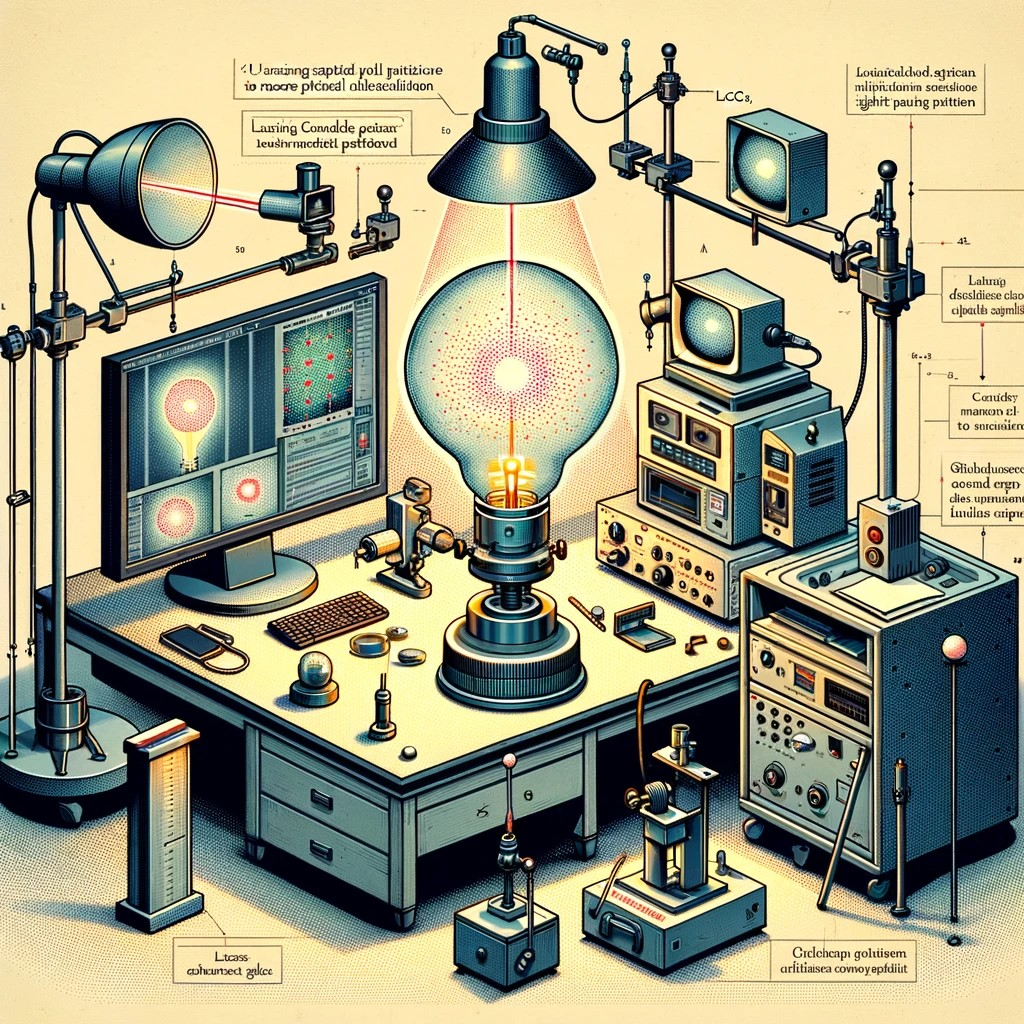
\includegraphics[width=0.3\textwidth]{Lab2_2Gra4.jpg}
			}
			\subfloat[]{
				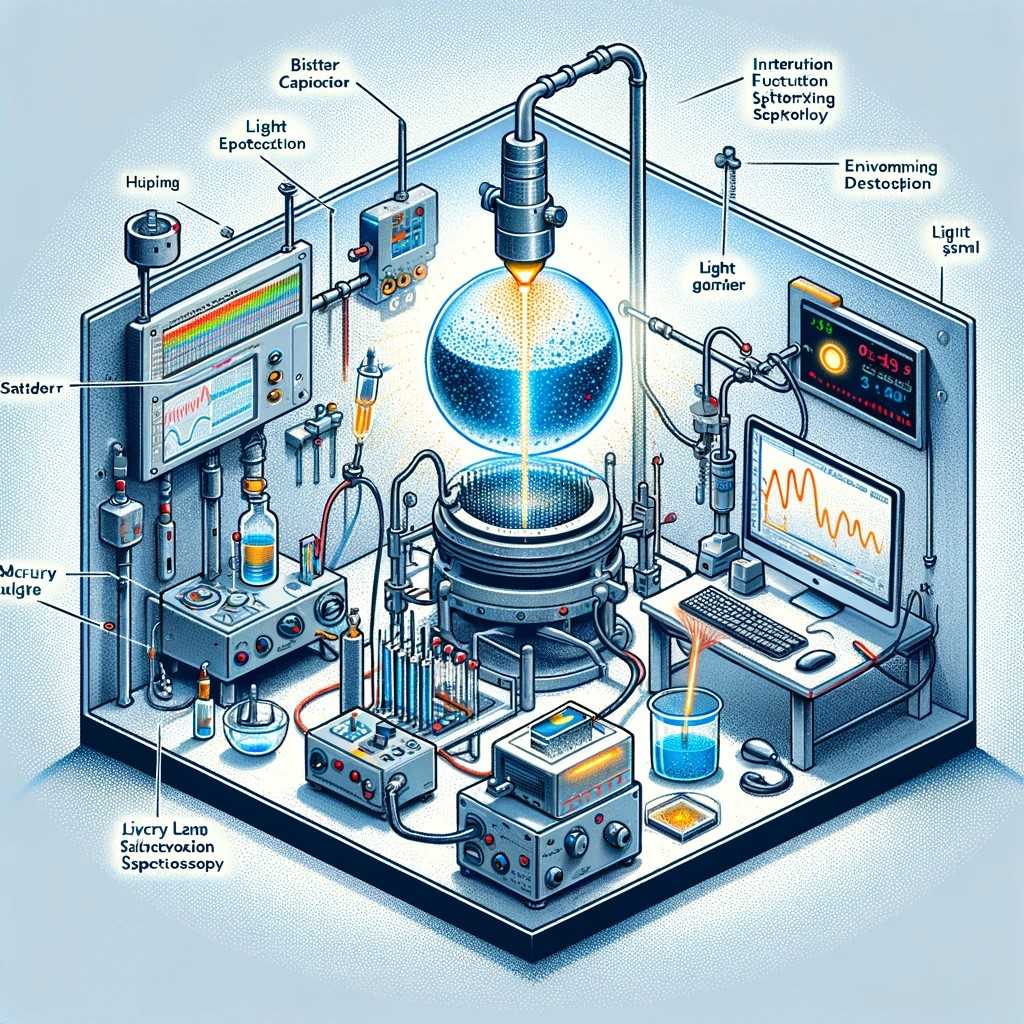
\includegraphics[width=0.3\textwidth]{Lab2_2Gra5.jpg}
			}
			\subfloat[]{
				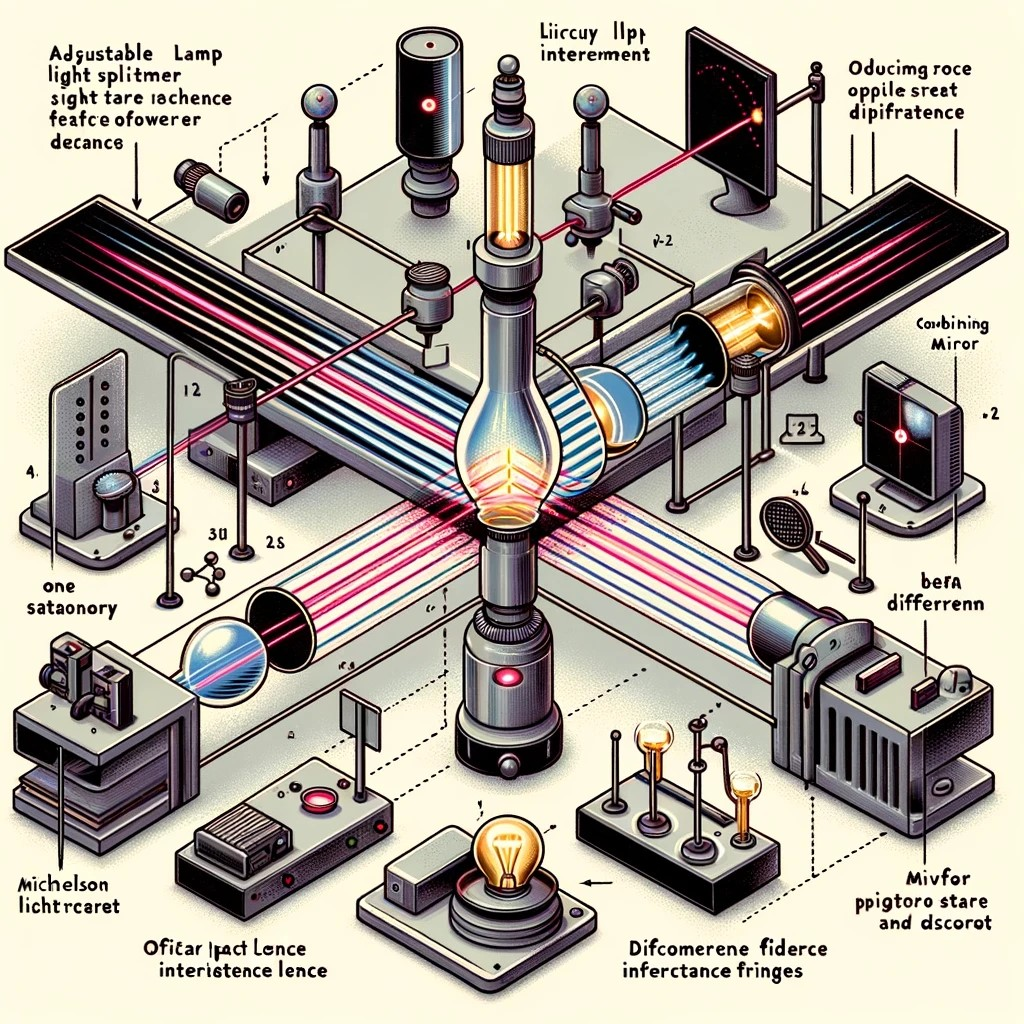
\includegraphics[width=0.3\textwidth]{Lab2_2Gra6.jpg}
			}
			\caption{迈克尔逊干涉仪光路图}
			\label{fig:fig4}			
		\end{figure}
		
		\item 方案设计1
		
		基于“使用散斑模式来测量空间相干性”的原理,我们可以设计如下的具体实验方案:
		
		\begin{enumerate}
			\item \textbf{实验目的}
			
			利用散斑模式测量汞灯光源的空间相干性,从而推算出相干长度。
			
			\item \textbf{所需材料}
			
			\begin{itemize}
				\item 汞灯光源
				\item 研磨玻璃
				\item CCD相机或高分辨率数码相机
				\item 光屏或投影屏
				\item 光学台及固定支架
				\item 计算机及图像处理软件
			\end{itemize}
			
			\item \textbf{实验步骤}
			
			\begin{enumerate}
				\item 光源准备:将汞灯安装在光学台上,使用合适的支架固定,确保光源稳定发光。
				\item 设置研磨玻璃:在汞灯光源前放置一块研磨玻璃,作为随机非均匀介质,用于产生散斑模式。研磨玻璃的粗糙度应适中,既能有效散射光线,又不至于使散斑过于模糊。
				\item 散斑捕获:在研磨玻璃的另一侧放置CCD相机或数码相机,对准研磨玻璃,以捕获散斑图案。相机应设置在适当的曝光和焦距下,以确保散斑图案的清晰度。
				\item 图像记录:开启汞灯,并通过相机记录下散斑图案。最好进行多次拍摄,以便于后续分析中对比和验证。
				\item 图像处理与分析:将捕获的散斑图案导入计算机,并使用图像处理软件进行分析。主要分析散斑尺寸和分布,这些特征与光源的空间相干性有直接关联。
				\item 相干性评估:根据散斑图案的特征,使用相关的理论和公式评估汞灯光源的空间相干性。空间相干性的评估可以通过比较实验散斑图案与理论模型进行,确定光源的相干长度。
			\end{enumerate}
			
			\item \textbf{注意事项}
			
			\begin{itemize}
				\item 确保实验室环境稳定,避免由于震动等因素引入额外的噪声。
				\item 实验中应注意光源的安全使用,避免直视强光。
				\item 实验数据的收集应尽量保持一致性,以便于数据分析时减少误差。
			\end{itemize}
			
		\end{enumerate}
		
		\item 方案设计2
		
		基于“强度波动光散射光谱学”测量相干性。
		
		\begin{enumerate}
			\item \textbf{实验目的}
			
			利用强度波动光散射光谱学法测量汞灯光源的空间和时间相干性,通过分析液晶样品散射光的强度波动来实现。
			
			\item \textbf{实验原理}
			
			强度波动光散射光谱学法基于分析液晶样品散射光的强度波动来探究光源的相干性。在此过程中,散射光的强度波动提供了光场空间和时间结构的信息,从而可以推断出光源的相干长度。
			
			\item \textbf{实验材料}
			
			\begin{itemize}
				\item 汞弧灯作为光源
				\item 液晶样品
				\item 散射室(以减小环境光干扰)
				\item 光强度检测系统(如光电探测器)
				\item 数据采集系统(如示波器或计算机配合数据采集卡)
			\end{itemize}
			
			\item \textbf{实验步骤}
			
			\begin{enumerate}
				\item 实验准备:将汞弧灯安置在散射室中,以减少环境光的影响。液晶样品放置在汞灯光源的光路中,以便光线可以通过样品并散射。
				\item 散射光的采集:使用光电探测器接收经液晶样品散射后的光,将探测器的输出信号传输至数据采集系统。
				\item 数据记录与分析:
				\begin{itemize}
					\item 记录散射光强度随时间的波动情况。
					\item 使用傅里叶变换等数学工具分析记录到的光强波动信号,提取相关的空间和时间相干性参数。
					\item 分析液晶样品散射光强度的统计特性,如强度分布和强度波动频谱。
				\end{itemize}
				\item 相干性评估:根据强度波动分析结果,评估汞灯光源的空间和时间相干性。特别是通过强度波动的统计特性来估算相干长度。
			\end{enumerate}
			
			\item \textbf{注意事项}
			
			\begin{itemize}
				\item 确保散射室内的环境光干扰尽可能小,以免影响实验结果。
				\item 在数据分析过程中,要注意选择合适的数学模型和分析方法,以确保结果的准确性。
				\item 根据实验结果调整光源和探测系统的参数,如需要,可以通过改变液晶样品的厚度或散射角度来优化实验设置。
			\end{itemize}
			
		\end{enumerate}
		
		\item \textbf{基于本实验实验原理设计方案}
		
		\begin{enumerate}
			\item \textbf{实验原理:}
			
			迈克尔逊干涉仪是一种典型的用于测量光的相干长度的仪器。其基本原理是将来自同一光源的光分成两束,让它们沿着不同的路径传播,然后再次合并。当两束光的路径差不超过光源的相干长度时,它们可以产生干涉图样。通过测量当干涉图样消失时的路径差,可以计算出光源的相干长度。
			
			\item \textbf{实验步骤:}
			
			\begin{enumerate}
				\item 准备实验装置:设置迈克尔逊干涉仪,包括一个可调节的汞灯光源、分束镜、两个反射镜(一个固定,一个可移动)、合束镜和观察屏或探测器。
				\item 调整光路:打开汞灯,通过调整迈克尔逊干涉仪中的分束镜和反射镜,使得两束光在合束镜处重合并形成干涉条纹。
				\item 测量干涉图样:通过缓慢移动一个反射镜,改变两束光之间的光程差。观察随着光程差的增加,干涉图样如何变化。
				\item 确定相干长度:记录当干涉条纹开始变得模糊直至消失的那一点的光程差。这个光程差即为两倍的相干长度(因为光程差包括往返两次的路径)。
				\item 计算相干长度:将记录的光程差除以2,得到汞灯光源的相干长度。
			\end{enumerate}
			
			\item \textbf{注意事项:}
			
			\begin{itemize}
				\item 在实验过程中,需要确保实验室内光线稳定,避免外部光线的干扰。
				\item 实验中应确保汞灯光源稳定,以避免测量误差。
				\item 由于汞灯光源的光谱可能包含多条谱线,可能需要通过滤光片选择特定的谱线进行测量。
			\end{itemize}
			
		\end{enumerate}
	\end{enumerate}
	
	
	% ---
	
	
	
	% 实验记录	
	\clearpage
	
	% 顶栏
	\begin{table}
		\renewcommand\arraystretch{1.7}
		\centering
		\begin{tabularx}{\textwidth}{|X|X|X|X|}
			\hline
			专业: & 物理学 & 年级: & 2022级 \\
			\hline
			姓名: & 杨舒云 & 学号: & 22344020\\
			\hline
			室温: &  & 实验地点: &  \\
			\hline
			学生签名:& 杨舒云 & 评分: &\\
			\hline
			实验时间:& 2024// & 教师签名:&\\
			\hline
		\end{tabularx}
	\end{table}
	% ---
	
	% 小标题
	\section{Lab2-2 迈克尔干涉实验(白光干涉)  \quad\heiti 实验记录}
	% ---
	
	% 实验过程记录
	\subsection{实验内容、步骤与结果}
	
	%
	\subsubsection{操作步骤记录}
	\begin{enumerate}
		\item 
	\end{enumerate}	
	
	%
	\subsubsection{}
	\begin{enumerate}
		\item \begin{table}[h]
			\centering
			\caption{表格示例}
			\label{tab:tab1}
			\begin{tabular}{|c|c|c|c|c|c|}
				\hline
				组1/序号i & 1 & 2 & 3 & 4 & 5 \\
				$v_{1i}(m/s)$ & 1.26 & 1.08 & 1.00 & 0.75 & 0.38 \\
				$f_{1i}(Hz)$ & 40073 & 40127 & 40105 & 40088 & 40066 \\
				\hline
				组2/序号i & 1 & 2 & 3 & 4 & 5 \\
				$v_{2i}(m/s)$ & 1.21 & 1.06 & 0.99 & 0.52 & 0.57 \\
				$f_{2i}(Hz)$ & 40143 & 40125 & 40084 & 40080 & 40067 \\
				\hline
				组3/序号i & 1 & 2 & 3 & 4 & 5 \\
				$v_{3i}(m/s)$ & 1.15 & 0.98 & 0.78 & 0.59 & 0.36 \\
				$f_{3i}(Hz)$ & 40135 & 40115 & 40092 & 40070 & 40044 \\
				\hline
			\end{tabular}
		\end{table}		
	\end{enumerate}
	
	% ---
	
	% 原始数据
	\clearpage
	\subsection{原始数据记录}
	实验记录本上的原始数据见%\cref{}(签字)。
	
	实验台桌面整理见%\textbf{附件}部分(\cref{})。
	
	其它原始数据见%\cref{}。
	% ---
	
	% 问题记录
	\subsection{实验过程中遇到的问题记录}
	\begin{enumerate}
		\item 
	\end{enumerate}
	% ---
	
	
	
	% 分析与讨论	
	\clearpage
	
	% 顶栏
	\begin{table}
		\renewcommand\arraystretch{1.7}
		\begin{tabularx}{\textwidth}{|X|X|X|X|}
			\hline
			专业:& 物理学 &年级:& 2022级\\
			\hline
			姓名: & 杨舒云 & 学号:& 22344020\\
			\hline
			日期:& 2024// & 评分: &\\
			\hline
		\end{tabularx}
	\end{table}
	% ---
	
	% 小标题
	\section{Lab2-2 迈克尔干涉实验(白光干涉) \quad\heiti 分析与讨论}
	% ---
	
	% 数据处理
	\subsection{实验数据分析}
	
	%
	\subsubsection{}
	\begin{enumerate}
		\item 
	\end{enumerate}
	
	%
	\subsubsection{}
	\begin{enumerate}
		\item 
	\end{enumerate}
	
	%
	\subsubsection{}
	
	% ---
	
	% 实验后思考题
	\subsection{实验后思考题}
	
	%思考题1
	\begin{question}
		
	\end{question}
	
	% 思考题2
	\begin{question}
		
	\end{question}
	
	% 思考题3
	\begin{question}
		
	\end{question}
	
	% ---
	
	
	% 结语部分
	\clearpage
	
	% 小标题
	\section{Lab2-2 迈克尔干涉实验(白光干涉) \quad\heiti 结语}
	% ---
	
	% 总结、杂谈与致谢
	\subsection{总结、杂谈与致谢}
	\begin{enumerate}
		\item 
	\end{enumerate}
	% ---
	
	% 参考文献
	\subsection{参考文献}
	[1] 维基百科 https://zh.wikipedia.org
	
	[2] 沈韩.基础物理实验.——北京:科学出版社,2015.2 ISBN:978-7-03-043311-4
	
	% ---
	
	% 附件
	\subsection{附件}
	试验台桌面整理如%\cref{}所示。
	
	实验报告个人签名如\cref{fig:name}。
	
	\begin{figure}[htbp]
		\centering
		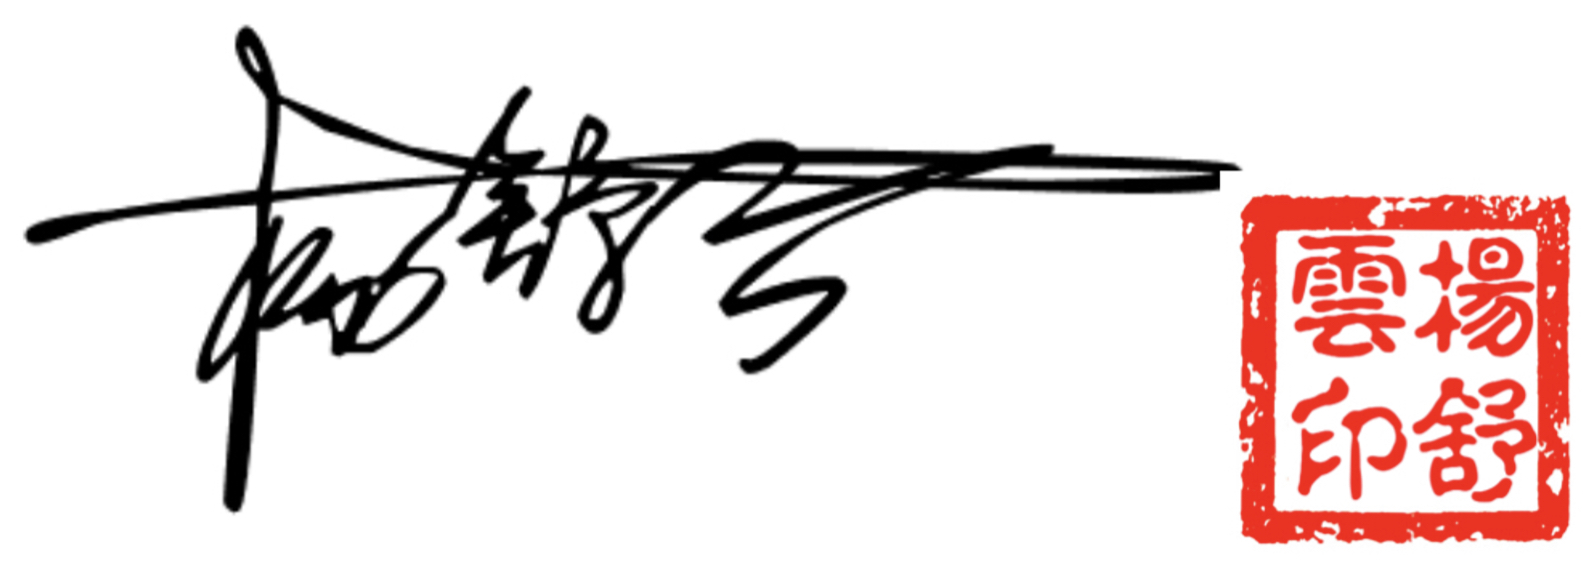
\includegraphics[width=0.7\textwidth]{name.png}
		\caption{个人签名}
		\label{fig:name}
	\end{figure}
	
	% ---
	
	相关代码已上传至Github。
	
	
	
\end{document}